\begin{center} 
\emph{``Most of the fundamental ideas of science are essentially simple, and may, as a rule, be expressed in a language comprehensible to everyone.'' -- Albert Einstein}
\end{center}

\section{The Fundamental Theorem of Linear Algebra}\label{sec:fundamental}
%This section will serve to review many of the important topics we have studied this semester with an emphasis on linear transformations and their matrix representations. \\
%
\begin{Exam}
\item Let $A = \mtx{rrrrr}{-3&6&-1&1&-7\\1&-2&2&3&-1\\2&-4&5&8&-4}\sim \mtx{rrrrr}{1&-2&0&-1&3\\0&0&1&2&-2\\0&0&0&0&0}$. Thus, $\nul A$ is a 3-dimensional subspace of $\R^5$ and $\nullity A = 3$. Likewise, $\col A$ is a $2$-dimensional subspace of $\R^3$ and $\rank A = 2$.
\end{Exam}\vs

\begin{Exam}
\item Let $A = \mtx{rrrrr}{1&3&3&2&-9\\-2&-2&2&-8&2\\2&3&0&7&1\\3&4&-1&11&-8}\sim \mtx{rrrrr}{1&0&-3&5&0\\0&1&2&-1&0\\0&0&0&0&1\\0&0&0&0&0}$. Thus, $\nul A$ is a 2-dimensional subspace of $\R^5$ and $\nullity A = 2$. Also, $\col A$ is a 3-dimensional subspace of $\R^4$ and $\rank A = 3$. 
\end{Exam}\vs

The rank of any matrix is the number of pivot positions. Suppose that $A$ is an $m\times n$ matrix with $p$ pivots. Then $\rank A = p$. This also implies that the number of non-pivot columns in $A$ is $n-p$. Consider the homogeneous system $A\bb x = \bb 0$. The number of non-pivot columns is the same as the number of free variables in the homogeneous system. As we have also seen, each free variable corresponds to a basis element for $\nul A$. Thus, $\nullity A = n-p$. This proves the following important theorem.\\

\begin{Thm}[The Rank-Nullity Theorem] If $A$ is an $m\times n$ matrix, then 
\[\rank A + \nullity A = n.\]
\end{Thm}\vs


\begin{Exam} Let $A$ be a $7\times 9$ matrix. Suppose that $\nullity A = 2$. Then by the Rank-Nullity Theorem, $\rank A = 7$, that is, the mapping $\bb x \mapsto A\bb x$ is surjective.\\

Is it possible for a $6\times 9$ matrix $A$  to have $\nullity A = 2$? No, because this implies that $\rank A = 7$. This is a contradiction because $\rank A \le 6 = \dim \R^6$. In fact, the Rank-Nullity Theorem tells us that $\nullity A \ge 3$.
\end{Exam}\vs



By the Rank-Nullity Theorem, we know that
\[\rank A + \nullity A = n.\] Taking transposes, we all have 
\[\dim(\row A) + \dim(\nul(A^\top) ) = m.\] \vs

\begin{Rem} The space $\nul(A^\top)$ is often called the \textbf{left null space} of $A$ because it consists of all $ 1\times m$ row vectors $\bb x$ such that $\bb xA = \bb 0$.
\end{Rem}\vs

\begin{Thm} For a matrix $A$, $\rank A = \rank A^\top$, that is, the dimension of the column and row space of $A$ are the same. 
\end{Thm}
\begin{proof}
First, the $\rank A$ is equal to the number of pivot columns. Let $B$ be the row reduced echelon form of $A$. Then $\dim (\row A) = \dim (\row B)$, where the second dimension is the same as the number of nonzero rows. But this equals the number of pivots.
\end{proof}\vs

\thmrepeat{thm:nonsingular}{\emph{(The Nonsingular Matrix Theorem--Continued)} Let $A$ be a square $n\times n$ matrix. Then the following statements are equivalent:
\begin{enumerate}[!THM!, start=1]
\begin{multicols}{2}
\item $A$ is a nonsingular matrix.\\
$\vdots$
\setcounter{enumi}{20}
\item $\col(A)=F^n$
\item $\nullity(A) = 0$
\item $\nul(A) = \bb 0$
\item $\corank(A) = n$
\item $\row(A)=F^n$
\item $\conullity(A) = 0$
\item $\lnl(A) = \bb 0$
\end{multicols}
\end{enumerate}
}

%\begin{Def} Let $T : F^n\to F^m$ be a linear transformation. The \textbf{adjoint} of $T$, denoted $T^*$ is the unique linear transformation $T^* : F^m\to F^n$ such that 
%\[T(\bb x) \cdot \bb y = \bb x \cdot T^*(\bb y),\qquad \forall \bb x\in F^n, \bb y\in F^m.\] A linear transformation $T:F^n \to F^n$ is called \textbf{self-adjoint} if $T^*=T$.
%\end{Def} \vs
%
%It is suspicious if even such a linear transformation exists, but rest assured; it does! If $A$ is an $m\times n$ matrix representation of $T$ with respect to the bases $\B\subseteq F^n$ and $\c\subseteq F^m$, then $T^*$ is the linear transformation represented by the matrix transpose $A^\top$ (or $A^*$, as appropriate) with respect to the bases $\c\to \B$. This is seen by the fact:
%\[T(\bb x)\cdot \bb y= (A\bb x) \cdot \bb y (A\bb x)^\top\bb y = (\bb x^\top A^\top)\bb y = \bb x^\top(A^\top\bb y) = \bb x\cdot (A^\top\bb y) = \bb x\cdot T^*(\bb y).\] Of course, the above identity also holds if the transpose $^\top$ is replaced with the conjugate transpose $^*$. Thus, the self-adjoint linear transformations are those represented by symmetric and Hermitian matrices.\\
%
%%\begin{Def} A \textbf{linear functional} is a linear transformation of the form $F^n \to F$. \end{Def}\vs
%%
%%Linear functionals are very special types of linear transformations, those which output just a scalar. For examples, let $\bb u\in F^n$ and define the map $T : F^n \to F$ by the rule $T(\bb v) = \bb u\cdot \bb v$ for all $\bb v\in F^n$. Properties of the inner product guarantee that this is a linear functional. Conversely, every linear functional has such a representation as an inner product of a fixed vector.\\
%%
%%\begin{Thm}[Riesz Representation Theory] Let $T : F^n \to F$ be a linear functional. Then there exists a vector $\bb u\in F^n$ such that $T(\bb v) = \bb u\cdot \bb v$ for all $\bb v\in F^n$.
%%\end{Thm}
%%\begin{proof}
%%Let $A$ be the standard matrix representation of $T$, which is a $1\times n$ matrix, that is, a row vector. Let $\bb u = A^\top\in F^n$. Then $T(\bb v) = A\bb v= (A^\top)^\top\bb v = \bb u^\top\bb v = \bb u\cdot \bb v$.
%%\end{proof}\vs
%%
%%Our take away from the Riesz Representation Theory is that while column vectors are the vectors in $F^n$, row vectors are their adjoints, that is, row vectors are the linear functionals associated to the column vectors in $F^n$. Furthermore, for any linear transformation $T:F^n\to F^m$, if $P_i : F^m \to F$ is the forgetful map that only reports the $i$th coordinate, then their composite $P_i\circ T : F^n\to F$ is a linear functional. Thus, $P_i\circ T$ is the same as the inner product of some vector in $F^n$. This is why the formulas of linear transformations always look like linear combinations of the input variables, because each formula is just  an inner product of the $i$th row vector of $[T]$.\\
%
%Next we establish the four fundamental spaces of a linear transformation. Some of these will be a review.\\
%
%\begin{Def} Let $T : F^n\to F^m$ be a linear transformation. The four \textbf{fundamental spaces} of $T$ are:
%\begin{enumerate}[(a)]
%\item The \textbf{kernel} of $T$: $\ker(T) = \{\bb x\in F^n\mid T(\bb x) = \bb 0\} \le F^n$, $\dim \ker(T) = \nullity(T)$.\\
%\item The \textbf{image} of $T$: $\im(T) = \{T(\bb x) \mid \bb x\in F^n\} \le F^m$, $\dim \im(T) = \rank(T)$.\\
%\item The \textbf{coimage} of $T$: $\coim(T) = \im(T^*) \le F^n$, $\dim \coim(T) = \corank(T)$.\\
%\item The \textbf{cokernel} of $T$: $\coker(T) = \ker(T^*) \le F^m$, $\dim \coker(T) = \conullity(T)$.\\
%\end{enumerate}
%\end{Def}
%
%The cokernel essentially measures how much is a linear transformation not surjective (onto), much in the same way the kernel measures how much a linear transformation is not injective (one-to-one).\\
%
%\begin{Thm} A linear transformation $T: F^n\to F^m$ is onto if and only if $\coker(T) = \{\bb 0\}$.\end{Thm}\vs
%
%The fundamental spaces are so called because they are all subspaces of the domain and codomain of $T$. Note that $\ker T, \coim T \le F^n$ and $\im T, \coker T \le F^m$. \\

We establish the four fundamental spaces of an $m\times n$ matrix $A$. Say $A$ has $p$ pivots. We have seen already three of these four fundamental spaces many times already:\\
%We have seen already three of these four fundamental spaces many times already. Let $A$ be a $m\times n$ matrix representation of $T$. Say $A$ has $p$ pivots. Then
%\begin{enumerate}[(a)]
%\item $\ker(T) = \nul(A) = \{\bb x\mid A\bb x= \bb 0\}\le F^n$, the \textbf{null space} of $A$  (the set of column vectors which produce zero with $A$ when multiplied on the right), $\nullity(T) = \nullity(A) = \dim\nul(A) = n-p$.\\
%\item $\im(T) = \col(A) = \{A\bb x\mid \bb x\in F^n \}\le F^m$, the \textbf{column space} of $A$ (the span of the column vectors of $A$), $\rank(T) = \rank(A) = \dim\col(A) = p$.\\
%\item $\coim(T) = \row(A) = \{\bb y^\top\bb A\mid \bb y\in F^m \} = \col(A^\top)\le F^n$, the \textbf{row space} of $A$ (the span of the rows vectors of $A$), $\corank(T) = \corank(A) = \dim\row(A) = p$.\\
%\item $\coker(T) = \lnl(A) = \{\bb y^\top\mid \bb y^\top A=\bb 0^\top  \} = \nul(A^\top )\le F^m$, the \textbf{left null space} of $A$ (the set of row vectors which produce zero with $A$ when multiplied on the left), $\conullity(T) = \conullity(A) = \dim\lnl(A) = m-p$.\\
%\end{enumerate}
\begin{enumerate}[!DEF!, start=1]
\item $\nul(A) = \{\bb x\mid A\bb x= \bb 0\}\le F^n$, the \textbf{null space} of $A$  (the set of column vectors which produce zero with $A$ when multiplied on the right), $\nullity(T) = \nullity(A) = \dim\nul(A) = n-p$.\\
\item $\col(A) = \{A\bb x\mid \bb x\in F^n \}\le F^m$, the \textbf{column space} of $A$ (the span of the column vectors of $A$), $\rank(T) = \rank(A) = \dim\col(A) = p$.\\
\item $\row(A) = \{\bb y^\top \bb A\mid \bb y\in F^m \} = \col(A^\top )\le F^n$, the \textbf{row space} of $A$ (the span of the rows vectors of $A$), $\corank(T) = \corank(A) = \dim\row(A) = p$.\\
\item $\lnl(A) = \{\bb y\mid \bb y^\top A=\bb 0^\top \} = \nul(A^\top)\le F^m$, the \textbf{left null space} of $A$ (the set of row vectors which produce zero with $A$ when multiplied on the left), $\conullity(T) = \conullity(A) = \dim\lnl(A) = m-p$.\\
\end{enumerate}

The left null space essentially measures how much the column vectors of $A$ do not span $F^m$, much in the same way the null space measures how much the column vectors are not linearly independent. We have seen that for a matrix $A$, the columns of $A$ are linearly independent if and only if the null space of $A$ is trivial. More generally, the dimension of the null space of $A$, its nullity, measures the size of the null space but also counts the number of free variables in the linear system $A\bb x= \bb b$. This is, of course, the number of non-pivot columns $n-p$. Similarly, the columns of $A$ span $F^m$ if and only if the left null space of $A$ is trivial. More generally, the dimension of the left null space of $A$, its conullity, measures the size of the left null space but also counts the number of rows of zeros in the row-reduced echelon form $U$ of $A$. This is, of course, the number of non-pivot rows $m-p$. The presence of a row of zeros in $U$ allows the possibilities of inconsistent linear systems $A\bb x=\bb b$ and is dependent on the choice of $\bb b$. Essentially, the left null space is the subspace of $F^m$ of those vectors $\bb b$ which ``definitely'' make $A\bb x = \bb b$ inconsistent.\\

%NEW
\begin{Exam}\label{exam:lnl} Let $A = \mtx{rrr}{3&-3&-2\\-5&4&3\\1&-5&-2}$. Note that 
\[\mtx{ccc}{7 & 4 & -1} \mtx{rrr}{3&-3&-2\\-5&4&3\\1&-5&-2} = \mtx{ccc}{21-20-1 & -21 +16+5 & -14 + 12 + 2} = \mtx{ccc}{0&0&0} = \bb 0^\top.\] Therefore, $\bb b = \vr{7\\4\\-1}\in \lnl(A)$. Next, if we try to solve the linear system $A\bb x = \bb b$, we see that 
\[\mtx{rrr|r}{3&-3&-2&7\\-5&4&3&4\\1&-5&-2&-1} \sim \mtx{rrr|r}{1&-5&-2&-1\\3&-3&-2&7\\-5&4&3&4} \sim \mtx{rrr|r}{1&-5&-2&-1\\0&12&4&10\\0&-21&-7&-1} \]
\[\sim \mtx{rrr|r}{1&-5&-2&-1\\0&3&1&5/2\\0&3&1&1/7} \sim  \mtx{rrr|c}{1&-5&-2&-1\\0&3&1&5/2\\0&0&0&-33/14}\] Therefore, $A\bb x = \bb b$ is inconsistent, as was to be expected.
\end{Exam}\vs

For all the other fundamental spaces, we have an algorithm to find a basis for the subspace by row-reducing $A$. We provide one here. To find a basis for $\lnl(A)$, augment $A$ with the identity matrix $I_m$ (of the appropriate size) and row reduce the matrix $[ A \mid I_m]$. Let $U$ be the row-reduced echelon form of $A$ and let $E \in F^{m\times m}$ be a product of elementary matrices which transform $A$ into $U$. Then $[A\mid I_m] \sim [U \mid E]$. Suppose that $U$ has a row of zeros in $i$th row.  Let $\bb \varepsilon_i$ be the $i$th row of $E$. Since $EA = U$, the $i$th row of $U$ is factored as $\bb\varepsilon_iA$. As this is a row of zeros, $\bb\varepsilon_i\in \lnl(A)$. As $E$ is a nonsingular matrix, its set of row vectors is linearly independent, as is any subset of row vectors. Considering that $\dim\lnl(A) = \conullity(A) = m-p =$ the number of zero rows, this independent set of row vectors must be a basis for $\lnl(A)$.\\

%NEW
\begin{Exam} Continuing with \examref{exam:lnl}, 
\[[A\mid I_3] = \mtx{rrr|rrr}{3&-3&-2&1&0&0\\-5&4&3&0&1&0\\1&-5&-2&0&0&1} \sim \mtx{rrr|rrr}{1&-5&-2&0&0&1\\0&3&1&1/4&0&-3/4\\0&0&0&-1/4&-1/7&1/28}\]
Hence, the third row corresponds to a row of zeros. Thus, the row vector on the right side of the augmentation is a basis element of $\lnl(A)$, namely, $\vr{-1/4\\-1/7\\1/28}$. We could replace this vector in the spanning set with any nonzero scalar multiple, namely $\bb b= -28\vr{-1/4\\-1/7\\1/28} = \vr{7\\4\\-1}$. Thus, $\lnl(A) = \Span\{(7, 4, -1)\}$.
\end{Exam}\vs

We present next the Fundamental Theorem of Linear Algebra, which is essentially a summary of many important results.\\

\begin{Thm}[The Fundamental Theorem of Linear Algebra] Let $A$ be an $m\times n$ matrix in $F^{m\times n}$. Then every vector $\bb v\in F^n$ can be decomposed uniquely as a sum of vectors:
\[\bb v = \bb v_{\row(A)} + \bb v_{\nul(A)}\] where $\bb v_{\row(A)}\in \row(A)$ and $\bb v_{\nul(A)} \in \nul(A)$. In particular, $\row(A)^\perp = \nul(A)$. Furthermore, if $A\bb v = \bb b$, then $\bb v_{\row(A)}$ is the particular solution to the linear system $A\bb x=\bb b$ of shortest length and $\bb v_{\nul(A)}$ is a solution to the associated homogeneous system $A\bb x = \bb 0$. \\

Likewise, every vector $\bb w\in F^m$ can be decomposed uniquely as a sum of vectors:
\[\bb w = \bb w_{\col(A)} + \bb w_{\lnl(A)}\] where $\bb  w_{\col(A)}\in \col(A)$ and $\bb w_{\lnl(A)}\in \lnl(A)$. In particular, $\col(A)^\perp = \lnl(A)$. Furthermore, if $A^\top\bb w = \bb b$, then $\bb w_{\col(A)}$ is the particular solution to the linear system $A^\top\bb y=\bb b$ of shortest length and $\bb w_{\lnl(A)}$ is a solution to the associated homogeneous system $A^\top\bb y = \bb0$.\\

Finally, 
\[\rank(A) + \nullity(A) = n,\qquad \corank(A) + \conullity(A) = m,\qquad \rank(A) = \corank(A).\]
\end{Thm}

{\color{red} This image needs to be replaced as it was ripped from another textbook. Also, the notion needs to be congruent with our presentation here.}

\centerline{\includegraphics[scale=0.5]{Chapter4/images/ftla.png}}


%%%%%%%%%%%%%%%%%%%%%%%%%%%%Contributed by Tyler Bayn Fall 2018 %%%%%%%%%%%%%%%%%%%%%%%%%%%%%%%%%%%
%%%%%%%%%%%%%%%%%%%%%%%%%%%%%%%%%%%%%%%%%%%%%%%%%%%%%%%%%%%%%%%%%%%%%%%%%%%%%%%
\begin{center}
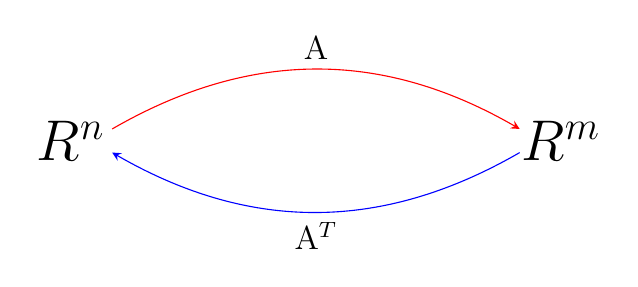
\begin{tikzpicture}[scale=0.75]
\node at (-4,0) {\huge $\mathbb{R}^{n}$};
\node at (4.3,0) {\huge $\mathbb{R}^{m}$};

\draw [->,>=stealth,red] (-3.3,0.2)  to [bend left]  node [above] {\large \textcolor{black}{A}}(3.6,.2);

\draw [<-,>=stealth,blue] (-3.3,-0.2) to [bend right] node [below] {\large \textcolor{black}{A$^{T}$}} (3.6,-0.2);

\end{tikzpicture}

%\hfill \break
%\hfill \break
%\hfill \break

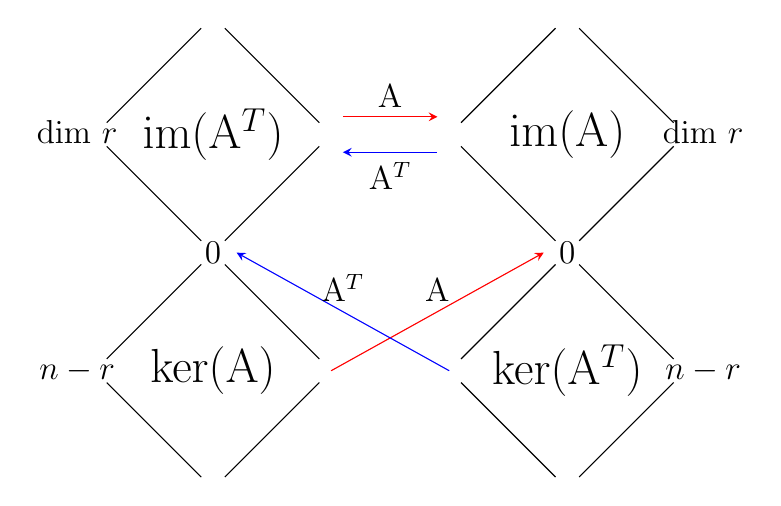
\begin{tikzpicture}[scale=0.75]
\draw (-4.8,2.2) -- (-3.2,3.8);
\draw (-2.8,3.8) -- (-1.2,2.2);
\draw (-4.8,1.8) -- (-3.2,0.2);
\draw (-2.8,0.2) -- (-1.2,1.8);

\draw (-4.8,-2.2) -- (-3.2,-3.8);
\draw (-2.8,-3.8) -- (-1.2,-2.2);
\draw (-4.8,-1.8) -- (-3.2,-0.2);
\draw (-2.8,-0.2) -- (-1.2,-1.8);

\draw (4.8,2.2) -- (3.2,3.8);
\draw (2.8,3.8) -- (1.2,2.2);
\draw (4.8,1.8) -- (3.2,0.2);
\draw (2.8,0.2) -- (1.2,1.8);

\draw (4.8,-2.2) -- (3.2,-3.8);
\draw (2.8,-3.8) -- (1.2,-2.2);
\draw (4.8,-1.8) -- (3.2,-0.2);
\draw (2.8,-0.2) -- (1.2,-1.8);

\draw [->,>=stealth,red] (-0.8,2.3) -- node [above] {\large \textcolor{black}{A}} (0.8,2.3);

\draw [<-,>=stealth,blue] (-0.8,1.7) -- node [below] {\large \textcolor{black}{A$^{T}$}} (0.8,1.7);

\node at (-3,0) {\large0};
\node at (3,0) {\large0};

\node at (-5.3,2.05) {\large dim $r$};
\node at (-5.3,-2) {\large $n - r$};
\node at (5.3,2.05) {\large dim $r$};
\node at (5.3,-2) {\large $n - r$};

\node at (-3,2) {\LARGE im(A$^{T}$)};
\node at (3,2) {\LARGE im(A)};
\node at (-3,-2) {\LARGE ker(A)};
\node at (3,-2) {\LARGE ker(A$^{T}$)};

\draw [->,>=stealth,red] (-1,-2) -- node [above] {\large \textcolor{black}{A}} (2.6,0);

\draw [->,>=stealth,blue] (1,-2) -- node [above] {\large \textcolor{black}{A$^{T}$}} (-2.6,0);

\end{tikzpicture}

\end{center}
%%%%%%%%%%%%%%%%%%%%%%%%%%%%%%%%%%%%%%%%%%%%%%%%%%%%%%%%%%%%%%%%%%%%%%%

%NEW
\begin{Exam} Solve the linear system $\begin{linear} 3x_1\ &-\ &3x_2\ &-\ &2x_3\ &=\ &3\\ -5x_1\ &+\ &4x_2\ &+\ &3x_3\ &=\ &-4\\ x_1\ &-\ &5x_2\ &-\ &2x_3\ &=\ &5 \end{linear}$ by finding the particular solution contained in the row space of the coefficient matrix.
\[\mtx{rrr|r}{3&-3&-2&3\\-5&4&3&-4\\1&-5&-2&5} \sim \mtx{rrr|r}{1&0&-1/3&0\\0&1&1/3&-1\\ 0&0&0&0}.\] Thus, the linear system is consistent and we see that 
\[\bb x = \vr{0\\-1\\0} + t\vr{1\\-1\\3},\] is the general solution to the linear system where $(1,-1,3)\in \nul(A)$. But $(0,-1,0) \notin \row(A)$. We know this since $(0,-1,0)\cdot (1,-1,3) = 1\neq 0$. On the other hand, we may solve the equation $\bb x_{\row(A)} \cdot (1,-1,3) = 0$. 
\[\bb x_{\row(A)} \cdot \vr{1\\-1\\3} =  \left(\vr{0\\-1\\0} + t\vr{1\\-1\\3}\right) \cdot \vr{1\\-1\\3} = \vr{0\\-1\\0}\cdot \vr{1\\-1\\3} + t\vr{1\\-1\\3}\cdot \vr{1\\-1\\3} = 0\]
\[(0+1+0) + t(1+1+9) = 0 \qRightarrow 1 + 11t = 0 \qRightarrow t = -\dfrac{1}{11}.\] Hence, $\bb x_{\row(A)} = \vr{0\\-1\\0} -\dfrac{1}{11}\vr{1\\-1\\3} = \vr{-1/11 \\ -10/11 \\ -3/11}$. It can be verified that $x_{\row(A)}$ is both a solution to the linear system and a member of $\row(A)$ (since it is orthogonal to $\nul(A)$).
\end{Exam}

%NEW
\begin{Exam} Solve the matrix equation $\mtx{rrrrr}{2&-6&0&0&0\\
3&-7&4&14&4\\
4&-19&-14&-49&-14\\
3&-6&6&21&6\\
-1&2&-2&-7&-2}\vr{x_1\\x_2\\x_3\\x_4\\x_5}=\mtx{c}{-72\\-78\\-249\\-63\\21}$ by finding the particular solution contained in the row space of the coefficient matrix.\\

We quickly solve the matrix equation $A\bb x=\bb b$. We do this by row reducing the augmented matrix $[A\mid \bb b]$ to RREF. We then grab the particular solution associated to setting all free variables to zero and also grab the basis to the null space of the coefficient matrix from the RREF:
\[\mtx{rrrrr|c}{2&-6&0&0&0&-72\\
3&-7&4&14&4&-78\\
4&-19&-14&-49&-14&-249\\
3&-6&6&21&6&-63\\
-1&2&-2&-7&-2&21} \sim \mtx{rrrrr|r}{1&0&6&21&6&9\\0&1&2&7&2&15\\0&0&0&0&0&0\\0&0&0&0&0&0\\0&0&0&0&0&0}.\] Hence,
\[\nul(A) = \Span\left\{\vr{-6\\-2\\1\\0\\0}, \vr{-21\\-7\\0\\1\\0}, \vr{-6\\-2\\0\\0\\1}\right\}\] and 
\[\bb x = \vr{9\\15\\0\\0\\0} + r\vr{-6\\-2\\1\\0\\0} +s \vr{-21\\-7\\0\\1\\0}+ t\vr{-6\\-2\\0\\0\\1} = \mtx{c}{9-6r-21s-6t\\15-2r-7s-2t\\r\\s\\t}.\] To find the unique solution $\bb x_{\row(A)}\in \row(A)$, we utilize the fact that $\row(A)^\top = \nul(A)$. Hence, $\bb x_{\row(A)}$ will be orthogonal to each vector in the basis of $\nul(A)$:
\begin{multline*}
\begin{linear}
\bb x_{\row(A)}\cdot (-6,-2,1,0,0)\ &= \ &0\\
\bb x_{\row(A)}\cdot (-21,-7,0,1,0)\ &=\ &0\\
\bb x_{\row(A)}\cdot (-6,-2,0,0,1)\ &= \  &0
\end{linear}\sim \begin{linear}
 -6(9-6r-21s-6t)-2(15-2r-7s-2t)+r\ &=\ &0\\
 -21(9-6r-21s-6t)-7(15-2r-7s-2t)+s\ &=\ &0\\
 -6(9-6r-21s-6t)-2(15-2r-7s-2t)+t\ &=\ &0
\end{linear}\\
\sim \begin{linear}
41r\ &+\ &140s\ &+\ &40t\ &=\ &84\\
140r\ &+\ &491\ &+\ &140t\ &=\ &294\\
40r\ &+\ &140s\ &+\ &41t\ &=\ &84
\end{linear}
\end{multline*} Solving this linear system, we get
\[\mtx{ccc|c}{41&140&40&84\\140&491&140&294\\40&140&41&84} \sim \mtx{ccc|c}{1&0&0&\frac{84}{571}\\0&1&0&\frac{294}{571}\\0&0&1&\frac{84}{571}}.\] Therefore, \[\bb x_{\row(A)} = \vr{9\\15\\0\\0\\0} + \frac{84}{571}\vr{-6\\-2\\1\\0\\0} +\frac{294}{571} \vr{-21\\-7\\0\\1\\0}+ \frac{84}{571}\vr{-6\\-2\\0\\0\\1} = \dfrac{1}{571}\mtx{c}{-2043\\6171\\84\\294\\84}. \qedhere \]
\end{Exam}

%%%%%%%%%%%%%%%%%% Exercises %%%%%%%%%%%%%%%%%%%
\startExercises{fundamental}

\noindent For Exercises \ref{exer:fundmatrixparamstart}-\ref{exer:fundmatrixparamstop}, consider the matrix $A$ and the bases for two of its fundamental subspaces, e.g., $\col(A)$ and $\nul(A)$. How many rows and columns does $A$ have, that is, what parameters $m\times n$ describe $A$? 
\begin{enumerate}[!HW!, start=1]
\item\label{exer:fundmatrixparamstart} $\col(A) = \Span\left\{\vr{2\\1}, \vr{-1\\0}\right\},\quad \nul(A)=\Span\left\{\vr{1\\-2\\1\\0\\0}, \vr{-3\\4\\0\\1\\0}, \vr{-5\\0\\0\\0\\1}\right\}$ %Daven Triplett
\item $\col(A) = \Span\left\{\vr{2\\3\\0\\-2}, \vr{-2\\4\\0\\-1}, \vr{2\\-5\\6\\4}\right\},\quad \nul(A)=\Span\left\{\vr{0\\0\\0\\1}\right\}$ %Daven Triplett
\item $\row(A) = \Span\left\{\vr{1\\0\\1}, \vr{0\\1\\2}\right\},\quad \lnl(A)=\Span\left\{\vr{7\\1\\-2}\right\}$  %Daven Triplett
\item\label{exer:fundmatrixparamstop} $\row(A) = \Span\left\{\vr{1\\2}\right\},\quad \lnl(A)=\Span\left\{\mtx{c}{1\\0\\0\\-1/4}, \mtx{c}{0\\1\\0\\1/2}, \mtx{c}{0\\0\\1\\-3/4}\right\}$ %Daven Triplett
\end{enumerate}

\noindent For Exercises \ref{exer:lnlstart}-\ref{exer:lnlstop}, compute a basis for the left null space $\lnl(A)$ where $A$ is the matrix provided. Answers may vary.
\begin{enumerate}[!HW!, label=$\spadesuit$ \arabic*., ref=\arabic*]
\begin{multicols}{3}
\item\label{exer:lnlstart} $\mtx{rrr}{-3&2&1\\7&-6&-5\\-7&4&1}$ %NEW
\itemspade $\mtx{rr}{1&2\\3&4\\5&6\\7&8\\9&10}$ %NEW
\item\label{exer:lnlstop} $ \mtx{rrrrr}{2&-2&-24&-46&114\\8&-8&-26&-44&106\\-7&7&5&3&-4\\-2&2&10&18&-44}$ %NEW
\end{multicols}
\end{enumerate}

\noindent For Exercises \ref{exer:rowsolutionstart}-\ref{exer:rowsolutionstop}, solve the linear system $A\bb x=\bb b$ by finding a particular solution in the row space of the coefficient matrix, that is, find $\bb x_{\row(A)}$.
\begin{enumerate}[!HW!, label=$\spadesuit$ \arabic*., ref=\arabic*]
\begin{multicols}{2}
\item\label{exer:rowsolutionstart} $\mtx{rr}{2&3\\-4&-6}\vr{x_1\\x_2} = \vr{2\\-4}$ %NEW
\itemspade $\mtx{rrr}{1&0&-3\\-2&3&0\\-1&-2&7}\vr{x_1\\x_2\\x_3} = \vr{-8\\4\\16}$ %NEW
\end{multicols}
\item\label{exer:rowsolutionstop} $\mtx{rrrr}{6&6&1&5\\1&1&0&1\\-2&-2&-4&2\\0&0&-3&3}\vr{x_1\\x_2\\x_3\\x_4} = \vr{9\\2\\8\\9}$ %New
\end{enumerate}

%%%%%%%%%%%%%%%%%%% Footnotes %%%%%%%%%%%%%%%%%%%
 \mbox{}\vfill
 
\pagebreak